\documentclass[12pt,x11names,a4paper]{article}
%Preamble

\usepackage{comment}
\usepackage[utf8]{inputenc}
\usepackage{amsmath}
\usepackage{amssymb}
\usepackage{amsthm}
\usepackage{enumitem}
\usepackage{mathrsfs}
\usepackage{mathtools}
\usepackage{esvect}
\usepackage{xfp}
\usepackage{xparse}
\usepackage{array}
\usepackage{changepage}
\usepackage{pdfpages}
\usepackage[parfill]{parskip}
\usepackage{anyfontsize}
\usepackage{alphalph}
\usepackage{ulem}
\usepackage{cancel}
\usepackage[framemethod=tikz]{mdframed}
\usepackage{xargs}
\usepackage{siunitx}              


\usepackage{algorithm}
\usepackage{algorithmic}
\usepackage{matlab-prettifier}
\usepackage{textcomp}
\usepackage{listings}
\usepackage[dvipsnames,svgnames]{xcolor}
\usepackage{colortbl}
\usepackage{eso-pic}
\usepackage[a4paper, margin=24mm]{geometry}
\usepackage{float}
\usepackage[danish]{babel}
\usepackage{tikz}
\usetikzlibrary{matrix,calc}
\usetikzlibrary{arrows}
\usetikzlibrary{arrows.meta}
\usetikzlibrary{decorations.pathreplacing}
\usetikzlibrary{decorations.pathreplacing,calligraphy}
\usetikzlibrary{patterns}
\usetikzlibrary{angles, quotes}
\usepackage{csquotes}
\usepackage{pdfpages}
\usepackage{fancyhdr}
\usepackage{lastpage}
\usepackage{pgfplots}
\usepackage{pgffor}

%Ændre følgende, hvis du vil have en anden bredde på pgfplots
\pgfplotsset{width=10cm,compat = 1.9}




\usepackage{caption}
\usepackage{subcaption}
\makeatletter
% \def\@seccntformat#1{%
%   \expandafter\ifx\csname c@#1\endcsname\c@section\else
%   \csname the#1\endcsname\quad
%   \fi}
 \makeatother
\counterwithin*{equation}{section}
\numberwithin{equation}{section}



%\newtheorem{setn}{Sætning}[section]
%\newtheorem{prop}[defn]{Proposition}
%\newtheorem{lem}[defn]{Lemma}
%\newtheorem{cor}[defn]{Korollar}

\newcommand\Tr{\textnormal{Tr}}
\newcommand\N{\textnormal{N}}
\newcommand{\suco}[2]{\left.#1\right|_{\mathbb{F}_{#2}}}
\renewcommand\qedsymbol{$\blacksquare$}
\theoremstyle{definition}
%\newtheorem{defn}[setn]{Definition}

\newcommand\Ker{\textnormal{Ker}\hspace{0.5mm}}
\renewcommand\Im{\textnormal{Im}\hspace{0.5mm}}
\newcommand\TS{\hspace{0.8mm}}

\usepackage{tcolorbox}
\tcbuselibrary{theorems}

\newmdtheoremenv[
	skipabove = 5pt,
	skipbelow = 5pt,
	roundcorner = 5,
	backgroundcolor = SeaGreen!30,
	linecolor = white, 
	]
	{defn}{Definition}[section]

\newmdtheoremenv[
	skipabove = 5pt,
	skipbelow = 5pt,
	roundcorner = 5,
	backgroundcolor = Melon!25,
	linecolor = white, 
	]
	{setn}[defn]{Sætning}
	
\newmdtheoremenv[
	skipabove = 5pt,
	skipbelow = 5pt,
	roundcorner = 5,
	backgroundcolor = Melon!25,
	linecolor = white, 
	]
	{lem}[defn]{Lemma}

\newtheorem{eksempel}[defn]{Eksempel}

\newenvironment{exa}
	{\begin{eksempel}}
	{\unskip\hfill $\square$ \end{eksempel}}
\newtheorem{regel}[defn]{Regel}


\usepackage{graphicx}
\usepackage[backend=biber]{biblatex}
\addbibresource{biblio.bib}

\renewcommand{\mod}[1]{\ (\textnormal{mod }{#1})}
\newcommand{\fmod}[1]{\ \textbf{mod }{#1}}
\usepackage{hyperref, bookmark}
\usepackage{booktabs}
\usepackage{calc}
\usepackage[nottoc,numbib]{tocbibind} 
\usepackage{multirow,bigdelim}

\renewcommand{\arraystretch}{1.3}
\newcommand\intd{\textnormal{d}}
\newcommand\e{\textnormal{e}}




\newenvironment{opgavetekst}[1]
{
	\begin{minipage}[t]{0.15\textwidth}
	 	\textbf{ #1}
	\end{minipage}
	\begin{minipage}[t]{0.85\textwidth}
		\rule{\textwidth}{0.3mm} \\
}
{ 
\\	\end{minipage}
}

\newenvironment{meretekst}
{
	\begin{minipage}[t]{0.15\textwidth}
	 	\phantom{h}
	\end{minipage}
	\begin{minipage}[t]{0.85\textwidth}
}
{ 
\\	\end{minipage}
}

\newenvironment{delopgave}[1]
{
	\begin{minipage}[t]{0.15\textwidth}
		\phantom{\textbf{Opgave}}		
		\textbf{\symbol{\numexpr96+ #1})}
	\end{minipage}
	\begin{minipage}[t]{0.85\textwidth}

	\begin{minipage}[t]{\textwidth}
}{
\end{minipage}
\phantom{h}\\
\end{minipage}
}

\newcommand{\cis}{\textnormal{\hspace{0.5mm}cis}}
%\newcommand{opgavelinje}[1]{
%\begin{minipage}[t]{0.15\textwidth}
%\textbf{#1}
%\end{minipage} 
%\begin{minipage}[t]{\textwidth}
%\rule{0.81\textwidth}{0.3mm}
%\end{minipage}
%}





%Farver!
\definecolor{NorregGroen}{RGB}{0,105,78}





\newgeometry{margin=2cm}

\pagestyle{fancy}
\fancyhf{}

\rhead{Nørre Gymnasium\\2.x	
}
\cfoot{Side \thepage \hspace{1pt} af \pageref{LastPage}}

%Husk at rette modul og dato!
\lhead{Aflevering 4\\ Matematik A }%<---------------------------------------RET
\chead{4. december 2026}%<----------------------------------------------------RET


\begin{document}

%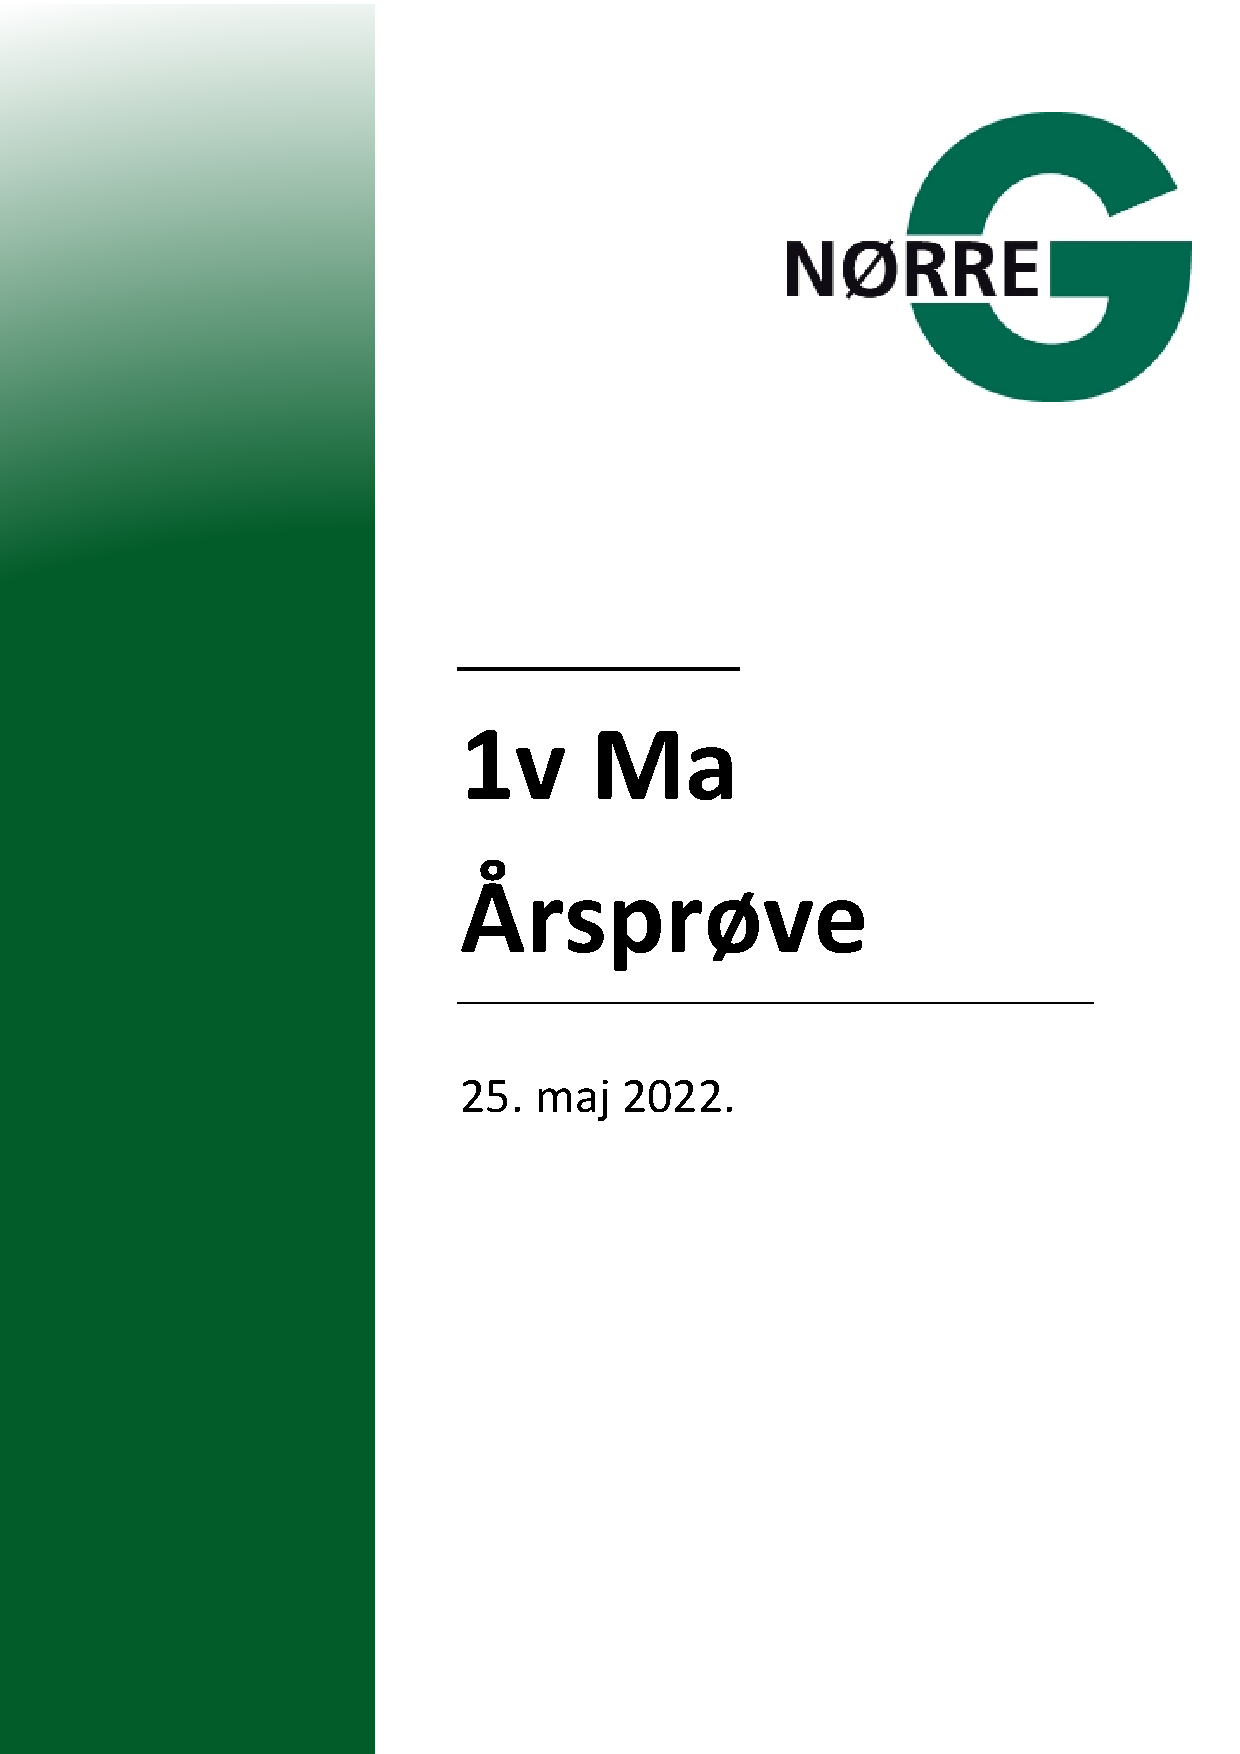
\includepdf[pages=-]{Forsider/aarsprove_1v.pdf}
\savegeometry{art}

\begin{titlepage}
\newgeometry{margin=0pt}

\begin{minipage}{0.27\textwidth}

\begin{tikzpicture}[overlay]
\fill[top color = NorregGroen!40, bottom color = NorregGroen] (6,10) rectangle (-10,-30);
\end{tikzpicture}
\end{minipage}
\begin{minipage}{0.73\textwidth}
\begin{center}
\phantom{h} \vspace{1cm}\\
\hspace{4cm}

\includegraphics[scale = 1]{Billeder/Norreg.png} \\
\phantom{h} \vspace{5cm}\\
\rule{0.7\textwidth}{0.3mm}\\
\phantom{h}\\
{\fontsize{50}{60}\selectfont Aflevering 4}\\%<---------------------------------------RET
\phantom{h}\\
\rule{0.7\textwidth}{0.3mm}\\
\Large 2026\\
\Large 2.x MA

\end{center}
\end{minipage}
\end{titlepage}
\loadgeometry{art}

%Udfyld afsnit herunder og lav til egen Latex-fil

%Kopier følgende til overskrift:

%\begin{center}
%\Huge
%Aflevering 1
%\end{center}
%\section*{Opgave 1}
%\stepcounter{section}
\begin{center}
%Opgavesætter er delt i to dele:\\
%Delprøve 1 kun med den centralt udmeldte formelsamling.\\
%Delprøve 2 med alle hjælpemidler.
\end{center}

\section*{Krav til formidling af din besvarelse}

Ved bedømmelse af helhedsindtrykket af besvarelsen af de enkelte opgaver lægges særlig vægt på følgende fire punkter:
\begin{itemize}
\item[$\cdot$] \textbf{Redegørelse og dokumentation for metode} \\
Besvarelsen skal indeholde en redegørelse for den anvendte løsningsstragegi med dokumentation i form af et passende antal mellemregninger \textit{eller} matematiske forklaringer på metoden, når et matematisk værktøjsprogram anvendes.
\item[$\cdot$] \textbf{Figurer, grafer og andre illustrationer} \\
Besvarelsen skal indeholde hensigtsmæssig brug af figurer, grafer og andre illustrationer, og der skal være tydelige henvisninger til brug af disse i den forklarende tekst.
\item[$\cdot$] \textbf{Notation og layout}\\
Besvarelsen skal i overensstemmelse med god matematisk skik opstilles med hensigtsmæssig brug af symbolsprog, og med en redegørelse for den matematiske notation, der indføres og anvendes, og som ikke kan henføres stil standardviden.
\item[$\cdot$] \textbf{Formidling og forklaring}\\
Besvarelsen af rene matematikopgaver skal indeholde en angivelse af givne oplysninger og korte forklaringer knyttet til den anvendte løsningsstrategi beskrevet med brug af almindelig matematisk notation. 

Besvarelsen af opgaver, der omhandler matematiske modeller, skal indeholde en kort præsentation af modellens kontekst, herunder betydning af modellens parametre. De enkelte delspørgsmål skal afsluttes med en præcis konklusion præsenteret i et klart sprog i relation til konteksten.
\end{itemize}

\newpage

\newpage\begin{center}
	\LARGE
	Uden hjælpemidler
\end{center}
\begin{opgavetekst}{Opgave 1}
	En funktion med forskriften 
	\begin{align*}
		f(x) = b\cdot a^x
	\end{align*}
	går gennem punkterne $(1,2)$ og $(5,32)$.
\end{opgavetekst}
\begin{delopgave}{1}
	Brug en formel til at finde tallene $a$ og $b$.
\end{delopgave}
\begin{delopgave}{2}
	Løs ligningen $f(x) = 8$.
\end{delopgave}
%
%
%
%
%
%
\begin{opgavetekst}{Opgave 2}
	Graferne $A$, $B$, $C$ og $D$ for fire funktioner $f$, $g$, $h$ og $\varphi$ givet ved
	\begin{align*}
		g(x) &= f(x + 3)	\\
		h(x) &= f(x - 3)\\
		\varphi(x) &= f(x) + 6\\
	\end{align*}		
	kan ses på Figur \ref{fig:parallelforskydning}.
	\begin{figure}[H]
	\centering
	\begin{tikzpicture}
	\begin{axis}[
		axis lines = center, xmin = -8, xmax = 7,
		ymin = -5, ymax = 35,
		xlabel = $x$, ylabel = $y$,
		ticks = none
		]
			\addplot[color = teal, thick, samples = 500, domain = -8:7] {x^2 + 2*x - 1};
			\addplot[color = olive, thick, samples = 500, domain = -8:7] {(x-3)^2 + 2*(x-3) - 1};
			\addplot[color = Melon, thick, samples = 500, domain = -8:7] {(x+3)^2 + 2*(x+3) - 1};
			\addplot[color = purple, thick, samples = 500, domain = -8:7] {x^2 + 2*x +19};
			\node[color = Melon] at (axis cs: -6,5) {$A$};
			\node[color = Teal] at (axis cs: -3,5) {$B$};
			\node[color = olive] at (axis cs: 4,5) {$C$};
			\node[color = purple] at (axis cs: 2,22) {$D$};
	\end{axis}
	\end{tikzpicture}
	\caption{Graferne $A$, $B$, $C$ og $D$.}
	\label{fig:parallelforskydning}
	\end{figure}
	\phantom{h}
\end{opgavetekst}
\begin{delopgave}{1}
	Afgør, hvilke af graferne $A$, $B$, $C$ og $D$ der tilsvarer funktionerne $f$, $g$, $h$ og $\varphi$. Begrund dit 
	svar. 
\end{delopgave}
%
%
%
%
%
\begin{opgavetekst}{Opgave 3}
	Grafen for en funktion $f$ kan ses på Figur \ref{fig:invers}.
\begin{figure}[H]
	\centering
	\begin{tikzpicture}
	\begin{axis}[
	axis lines = center, 
	xmin = -2.5, xmax = 7.5,
	ymin = -2.5, ymax = 7.5,
	xlabel = $x$, 
	ylabel = $y$,
	xtick = {-4,-2,...,6,8},
	ytick = {-4,-2,...,6,8},
	minor tick num = 1,
	grid = both,
	]
		\addplot[color = olive, thick, samples = 500, domain = 0:10] {x^2-2};
	\end{axis}
	\end{tikzpicture}
	\caption{Grafen for $f$.}
	\label{fig:invers}
\end{figure}
\phantom{h}
\end{opgavetekst}
\begin{delopgave}{1}
	Bestem $f^{-1}(-2)$
\end{delopgave}
\begin{delopgave}{2}
	Løs ligningen $f(x) = 7$
\end{delopgave}
\begin{delopgave}{2}
	Løs ligningen $f^{-1}(x) = 2$
\end{delopgave}

%
%
%
%
%
\begin{opgavetekst}{Opgave 4}
En trekant $\triangle ABC$ kan ses på Figur \ref{fig:trekantareal}

\begin{figure}[H]
	\centering
	\begin{tikzpicture}
		\draw[color = olive, thick] (-7,0) -- (0,0) node[midway, anchor = south] {$5$};
		\draw[color = olive, thick] (-5.2,-3) -- (0,0) node[midway, anchor = north west] {$6$};
		\draw[color = olive, thick] (-7,0) -- (-5.2,-3) node[midway, anchor = east] {$c$};
		\draw[color = olive, thick] (-0.7,0) arc (180:210:0.7) node[midway, anchor = east] {$30^{\circ}$};
		\node[color = olive, anchor = east] at (-7,0) {$A$};
		\node[color = olive, anchor = west] at (0,0) {$C$};
		\node[color = olive, anchor = north] at (-5.2,-3) {$B$};
	\end{tikzpicture}
	\caption{Trekanten $\triangle ABC$.}
	\label{fig:trekantareal}
\end{figure}
\phantom{h}
\end{opgavetekst}
\begin{delopgave}{1}
	Bestem arealet af trekant $\triangle ABC$ ved at bruge Tabel \ref{tab:cossintan} i bilaget.
\end{delopgave}
%
%
%
%
%
\newpage
\begin{opgavetekst}{Opgave 5}
	En funktion $g$ er givet ved
	\begin{align*}
		g(x) = x^4-72x^2 + 19
	\end{align*}
\end{opgavetekst}
\begin{delopgave}{1}
	Bestem forskriften for funktionen 
	\begin{align*}
		\frac{dg}{dx}.
	\end{align*}
\end{delopgave}
\begin{delopgave}{2}
	Bestem ekstremumsstederne for $g$. 
\end{delopgave}
%
%
%
%
%
\begin{opgavetekst}{Opgave 6}
Trekanten $\triangle ABC$ kan ses på Figur \ref{fig:trekantcos}.
	\begin{figure}[H]
		\centering
		\begin{tikzpicture}
		%A
		\pgfmathsetmacro{\ax}{0}
		\pgfmathsetmacro{\ay}{0}
		%B
		\pgfmathsetmacro{\bx}{5}
		\pgfmathsetmacro{\by}{2}
		%C
		\pgfmathsetmacro{\cx}{7}
		\pgfmathsetmacro{\cy}{0}
		%arc radius
		\pgfmathsetmacro{\arclen}{0.7}
		%c
		\draw[color = olive, thick] (\ax,\ay) -- (\bx,\by) node[midway, anchor = south east] {$5$};
		%b
		\draw[color = olive, thick] (\ax,\ay) -- (\cx,\cy) node[midway, anchor = north] {$6$};
		%a
		\draw[color = olive, thick] (\bx,\by) -- (\cx,\cy) node[midway, anchor = south west] {$2$};
	%	Vinkel A		
		\draw[color = olive, thick] (\arclen,0) arc (0:21.8:\arclen) 
		node[midway, anchor = west] {};
	%	Vinkel B
		\draw[color = olive, thick] (4.35,1.74) arc (180 + 21.8:180 + 21.8 + 113.2:\arclen)
		 node[midway, anchor = north east] {};
	%	Vinkel C
		\draw[color = olive, thick] (\cx - \arclen,0) arc (180:180 - 45:\arclen)
		 node[midway, anchor = east] {};
		 %Nodes
		 \node[color = olive, anchor = east] at (\ax,\ay) {$A$};
		 \node[color = olive, anchor = south] at (\bx,\by) {$B$};
		 \node[color = olive, anchor = west] at (\cx,\cy) {$C$};
		\end{tikzpicture}
		\caption{Trekanten $\triangle ABC$.}
		\label{fig:trekantcos}
	\end{figure}
	\phantom{h}
\end{opgavetekst}
\begin{delopgave}{1}
	Bestem vinklen $\angle B$. Brug Tabel \ref{tab:cossintan} hvor du afrunder til to decimaler. 
\end{delopgave}

\begin{opgavetekst}{Opgave 7}
	En funktion $h$ er givet ved
	\begin{align*}
		h(x) = x^2 -2x + k
	\end{align*}
\end{opgavetekst}
\begin{delopgave}{1}
	Bestem det sted, hvor tangenten for $h$ har hældningen $6$.
\end{delopgave}
\begin{delopgave}{2}
	Bestem tallet $k$ så tangenten i dette punkt har ligningen
	\begin{align*}
		y = 6x - 20.
	\end{align*}
\end{delopgave}
\newpage
\begin{center}
	\LARGE
	Med hjælpemidler
\end{center}
\begin{opgavetekst}{Opgave 8}
	\begin{center}
		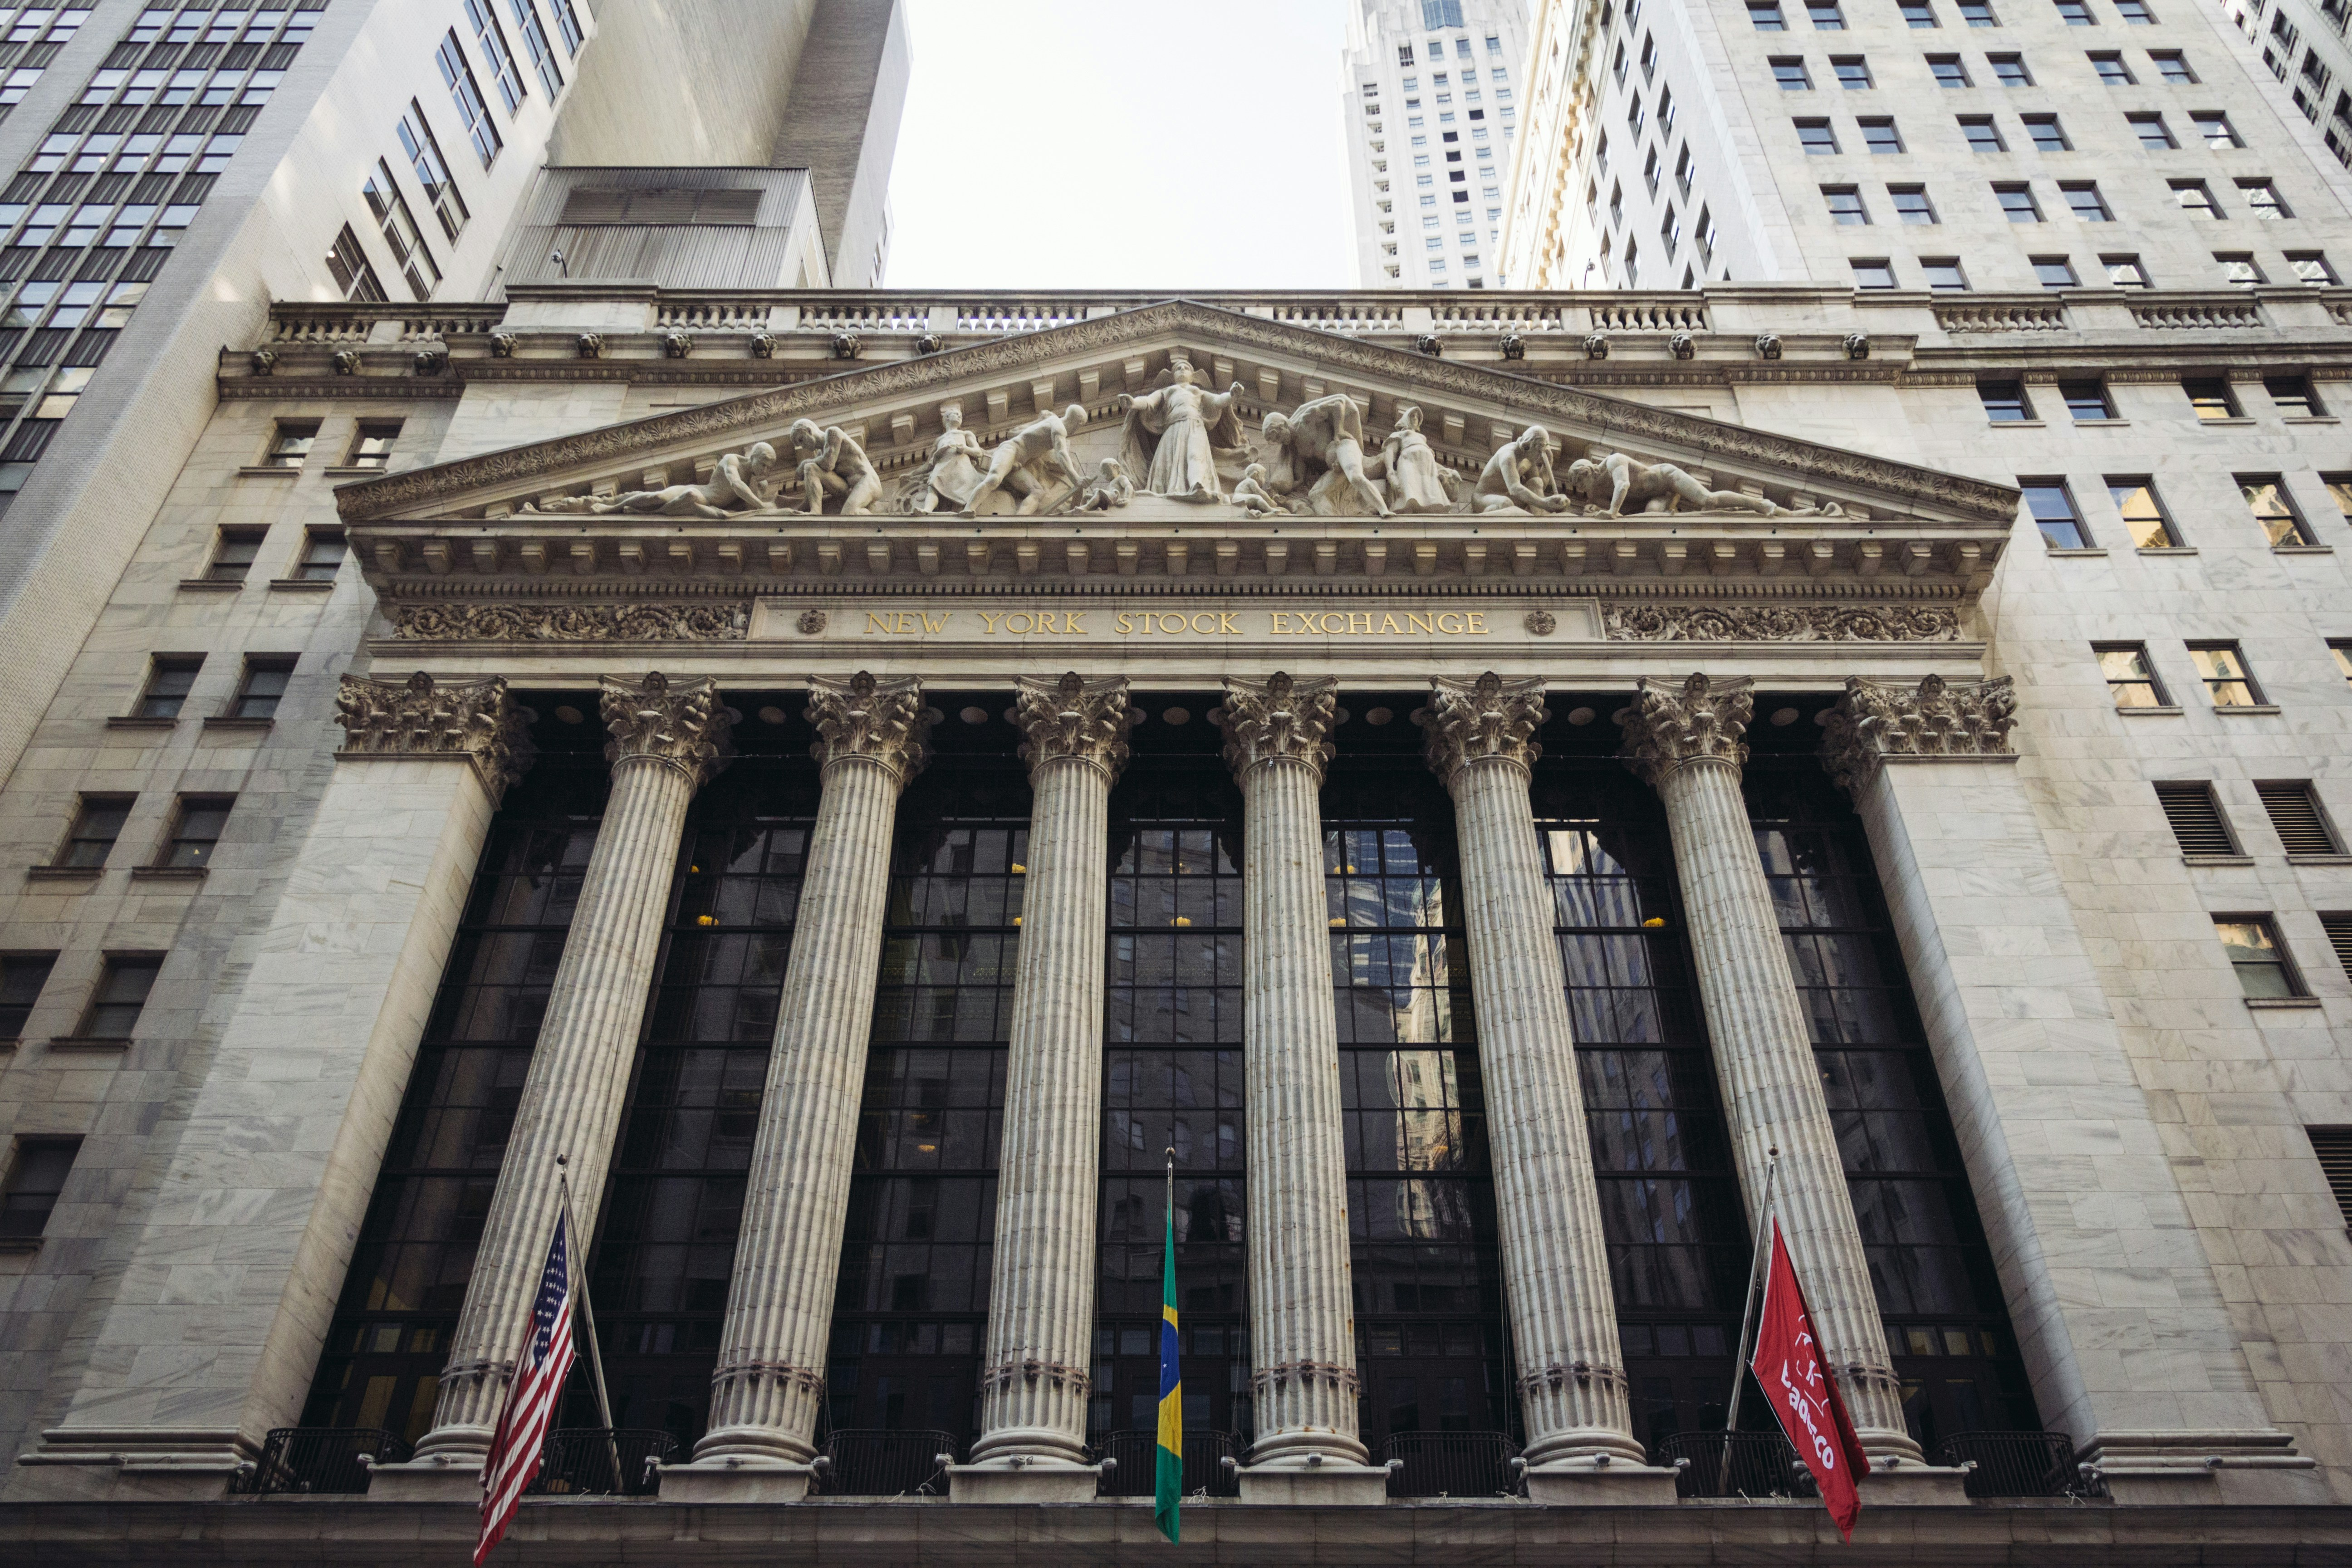
\includegraphics[width=0.6\textwidth]{Billeder/NYstockexchange}
	\end{center}
	S$\&$P 500-indekset er et aktieindeks, der følger 500 af de største virksomheder i USA. I \href{https://github.com/ChristianJLex/TeachingNotes/raw/master/2025-2026/Data%20og%20lign/SnP500.xlsx}{\color{blue!60} dette datasæt} ses 
	indeksets værdi siden 1988.
	
	Det antages, at indeksets værdi kan beskrives ved en sammenhæng af typen
	\begin{align*}
		P(t) = b\cdot a^t,
	\end{align*}
	hvor $P$ betegner værdien af indekset i USD og $t$ betegner det forløbne antal år siden 1978.
\end{opgavetekst}
\begin{delopgave}{1}
	Brug datasættet til at bestemme en forskrift for $P$. 
\end{delopgave}
\begin{delopgave}{2}
	Bestem $\frac{dP}{dt}$ til $t = 37$ og giv en fortolkning af tallet.
\end{delopgave}
\begin{meretekst}
	Et andet indeks, der beskriver teknologivirksomheder har siden 1978 kunne beskrives ved
	\begin{align*}
		Q(t) = 10.11\cdot 1.143^t,
	\end{align*}
	hvor $t$ er den forløbne tid efter 1978 og $Q$ er prisen på indekset i USD.
\end{meretekst}
\begin{delopgave}{3}
	Tegn graferne for $P$ og $Q$ i samme koordinatsystem så $t \in [0,60]$
\end{delopgave}
\begin{delopgave}{4}
	Bestem det årstal, hvor prisen på $Q$ vokser hurtigere end prisen på $P$. 
\end{delopgave}
%
%
%
%
%
\begin{opgavetekst}{Opgave 9}
	\begin{center}
		
\includegraphics[width=0.6\textwidth]{Billeder/tiktok}
	\end{center}
	I Tabel \ref{tab:tiktok} kan antal brugere af videodelingsappen TikTok henover en årrække ses. 
	\begin{table}[H]
		\centering
		\rowcolors{1}{olive!25}{olive!10}
		\begin{tabular}{ccccccccc}
		Årstal & 2018 & 2019 & 2020 & 2021 & 2022 & 2023 & 2024 & 2025 \\
		Brugere i mia. & 0.34 & 0.65 & 1.04 & 1.41 & 1.72 & 1.92 & 2.05 & 2.14
		\end{tabular}
		\caption{Antal brugere af appen TikTok på verdensplan.}
		\label{tab:tiktok}
	\end{table}
	Det antages, at antallet af brugere kan beskrives ved det, vi kalder en \textit{logistisk vækstkurve}. Skal man lave 
	logistisk regression i Maple, skriver man
	\begin{align*}
		&\texttt{with(Gym):}\\
		&\texttt{LogistReg(data)}
	\end{align*}	 
	\phantom{h}
\end{opgavetekst}
\begin{delopgave}{1}
	Brug tallene fra Tabel \ref{tab:tiktok} til at bestemme en logistisk model $f$, der beskriver antallet af TikTok-
	brugere som funktion af det forløbne antal år siden 2018.
\end{delopgave}
\begin{meretekst}
	Tiktok har en forhåbning om, at have 2.35 mia. brugere i år 2029.
\end{meretekst}
\begin{delopgave}{2}
	Brug din model til at afgøre, om dette mål er realistisk for TikTok.
\end{delopgave}
\begin{delopgave}{3}
	Bestem det tidspunkt, hvor antallet af brugere vokser hurtigst. 
\end{delopgave}
%
%
%%%%%%%%%%%%%%%
%
%


\newpage
\section*{Bilag}
\begin{table}[H]
	\centering
	\begin{tikzpicture}
	\node at (0,0) {$v$};
	\node at (2*0.9,0) {$\cos(v)$};
	\node at (4*0.9,0) {$\sin(v)$};
	\node at (6*0.9,0) {$\tan(v)$};
	\node at (8*0.9,0) {$v$};
	\node at (10*0.9,0) {$\cos(v)$};
	\node at (12*0.9,0) {$\sin(v)$};
	\node at (14*0.9,0) {$\tan(v)$};
	\scriptsize
	%Colors
	\foreach \i in {0,...,22}{
		\filldraw[color = teal!60, opacity = 0.4] (-0.9,-0.5-0.3+0.15-\i*0.3*2) rectangle
		 (14*0.9 + 0.9,-0.5-0.3-0.15-\i*0.3*2);
	}
	\foreach \i in {0,...,45}{
		%Macros for evaluating
		\pgfmathsetmacro{\cval}{cos(\i)}
		\pgfmathsetmacro{\sval}{sin(\i)}
		\pgfmathsetmacro{\tval}{tan(\i)}
		%First columns of values
		\node at (0,-0.5-\i*0.3) {$\i^{\circ}$};
		\node at (2*0.9,-0.5-\i*0.3) { \cval };
		\node at (4*0.9,-0.5-\i*0.3) { \sval };
		\node at (6*0.9,-0.5-\i*0.3) { \tval };
	}
	\foreach \i in {46,...,89}{
		%Macros
		\pgfmathsetmacro{\cval}{cos(\i)}
		\pgfmathsetmacro{\sval}{sin(\i)}
		\pgfmathsetmacro{\tval}{tan(\i)}
		%Second column
		\node at (8*0.9,-0.5-\i*0.3 + 46*0.3) {$\i^{\circ}$};
		\node at (10*0.9,-0.5-\i*0.3 + 46*0.3) { \cval };
		\node at (12*0.9,-0.5-\i*0.3 + 46*0.3) { \sval };
		\node at (14*0.9,-0.5-\i*0.3 + 46*0.3) { \tval };
	}
		\pgfmathsetmacro{\cval}{cos(90)}
		\pgfmathsetmacro{\sval}{sin(90)}
		\node at (8*0.9,-0.5-90*0.3 + 46*0.3) {$90^{\circ}$};
		\node at (10*0.9,-0.5-90*0.3 + 46*0.3) { \cval };
		\node at (12*0.9,-0.5-90*0.3 + 46*0.3) { \sval };
	\end{tikzpicture}
	\caption{Tabel over udvalgte værdier for $\cos$, $\sin$ og $\tan$.}
	\label{tab:cossintan}
\end{table}

\end{document}




